\documentclass[10pt,xcolor=pdflatex]{beamer}
\usepackage{newcent}
\usepackage[utf8]{inputenc}
%\usepackage[czech]{babel}
\usepackage{hyperref}
\usepackage{fancyvrb}
\usepackage{multicol}

\usetheme{FIT}

%%%%%%%%%%%%%%%%%%%%%%%%%%%%%%%%%%%%%%%%%%%%%%%%%%%%%%%%%%%%%%%%%%
\title{Continuous Integration and Automated Code Review in Open Source Projects}

\author[]{Adrián Tóth}

\institute[]{
    Brno University of Technology, Faculty of Information Technology\\
    Bo\v{z}et\v{e}chova 1/2. 612 66 Brno - Kr\'alovo Pole\\
    xtotha01@fit.vutbr.cz
    }

%\date{January 1, 2016}
%\date{\today}
\date{} % bez data

%%%%%%%%%%%%%%%%%%%%%%%%%%%%%%%%%%%%%%%%%%%%%%%%%%%%%%%%%%%%%%%%%%

\begin{document}

\frame[plain]{\titlepage}

\begin{frame}\frametitle{Introduction}
    \begin{center}
        \begin{tabular}{l}
            What is \textit{Continuous Integration}?\\[1em]
            What is \textit{Automated Code Review}?\\[1em]
            Where is it used and why?\\[1em]
            How it works?
        \end{tabular}
    \end{center}
\end{frame}

\begin{frame}\frametitle{Continuous Integration}
    \begin{itemize}
        \item common part of fast software development\\[1em]
        \item adaptive development technique\\[1em]
        \item reduce integration problems\\[1em]
        \item integrations are verified via automated tests and builds\\[1em]
        \item popular in open source projects which are frequently developed by a group of people\\[1em]
        \item available CI services: \textit{Travis CI}, \textit{Jenkins}, \textit{TeamCity}, ...
    \end{itemize}
\end{frame}

\begin{frame}\frametitle{Components of CI System}
    \begin{figure}[H]
        \centering
        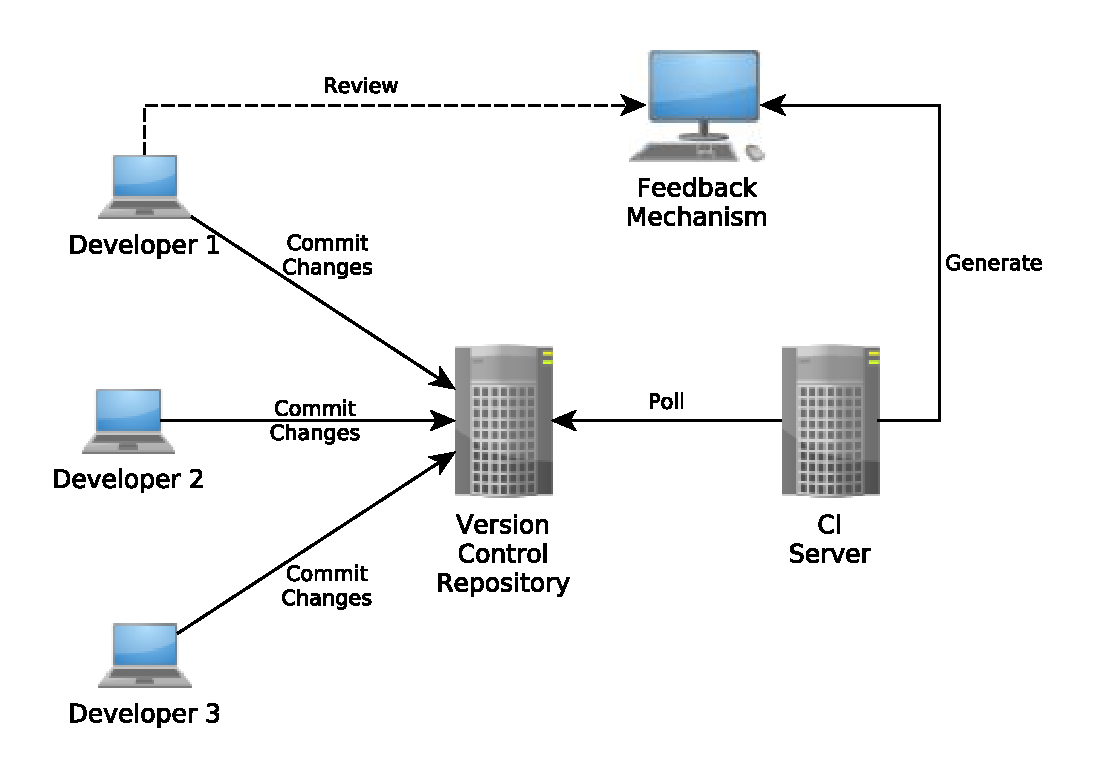
\includegraphics[scale=0.5]{eps/components_of_CI_system.eps}
    \end{figure}
\end{frame}

\begin{frame}\frametitle{Basics of CI}
    \begin{multicols}{2}
        Stages of CI:
        \begin{enumerate}
            \item Change
            \item Reaction
            \item Feedback
            \item Waiting 
        \end{enumerate}
        \begin{figure}[H]
            \centering
            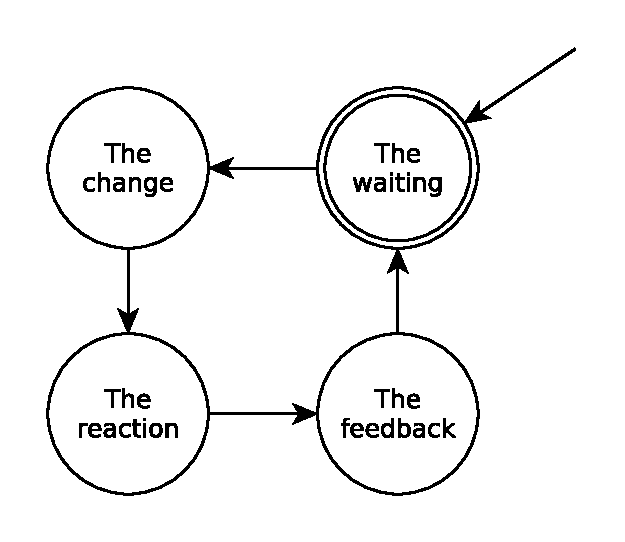
\includegraphics[scale=0.5]{eps/stages_of_ci.eps}
        \end{figure}
    \end{multicols}
\end{frame}

\begin{frame}\frametitle{Basics of CI}
    \begin{centering}
        \large{How it works?}\\[1em]
    \end{centering}
    \begin{figure}[H]
        \centering
        \hspace{-1.7em} 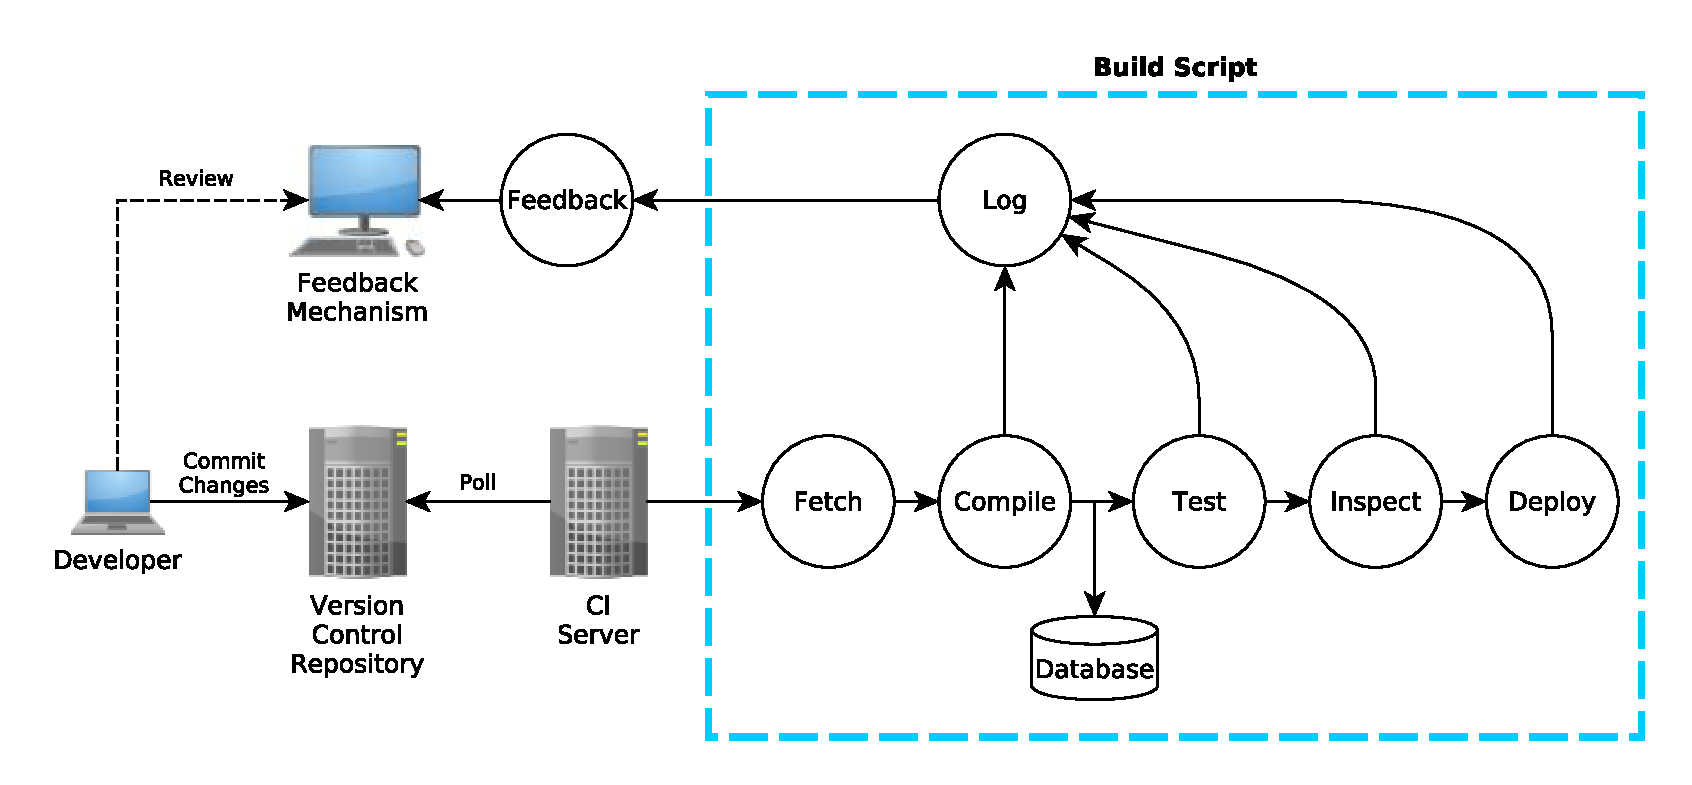
\includegraphics[scale=0.4]{eps/build_script.eps}
    \end{figure}
\end{frame}

\begin{frame}\frametitle{Code Review}
    Types of code review:\\[0.5em]
    \begin{itemize}
        \item manual code review
            \begin{itemize}
                \item[$\circ$] collaborative inspection and discussion with project members\\[0.25em]
                \item[$\circ$] slow (nearly 100 lines of code per hour)\\[0.25em]
                \item[$\circ$] pair programming\\[1em]
            \end{itemize}
        \item automated code review
            \begin{itemize}
                \item[$\circ$] \dots
            \end{itemize}
            
    \end{itemize}
\end{frame}

\begin{frame}\frametitle{Automated Code Review}
    \begin{itemize}
        \item inspection of code quality
            \begin{itemize}
                \item[$\circ$] coding standards
                \item[$\circ$] trailing spaces
                \item[$\circ$] code duplication
                \item[$\circ$] not enough / too many comments
                \item[$\circ$] \dots\\[1em]
            \end{itemize}
        \item detection of basic mistakes and vulnerabilities\\[1em]
        \item matching set of rules providing static analysis\\[1em]
        \item RuboCop, SonarQube, RIPS, FlexeLint
    \end{itemize}
\end{frame}

\begin{frame}\frametitle{Automated Code Review}
    TODO
\end{frame}

\begin{frame}\frametitle{Objectives}
    \begin{itemize}
        \item \textit{Pronto}\footnote{\color{cyan}\href{https://github.com/prontolabs/pronto}{github.com/prontolabs/pronto}} integration\\[0.5em]
        \item \textit{Webhooks}\footnote{\color{cyan}\href{https://developer.github.com/webhooks}{developer.github.com/webhooks}} integration\\[0.5em]
        \item Request for review command implementation\\[0.5em]
        \item \textit{Gitter} integration (yell if master is broken)\\[0.5em]
        \item \textit{Pull Request Processor}\footnote{\color{cyan}\href{https://github.com/theforeman/prprocessor}{github.com/theforeman/prprocessor}} integration\\[0.5em]
        \item \textit{Github Status API}\footnote{\color{cyan}\href{https://developer.github.com/v3/repos/statuses}{developer.github.com/v3/repos/statuses}} integration\\[0.5em]
        \item Track dependent pull requests (comment if merged)
    \end{itemize}
\end{frame}

\bluepage{Thank You For Your Attention !}

\end{document}
